\chapter{Acquisition-System Design}
\section{Overview}
The first step after understanding the basic theory behind microphone arrays and beamforming is to apply this knowledge in a practical setting.
The primary goal is to record and analyze real-world audio data from a variety of microphones.
This involves the evaluation of different microphone types and array configurations.
Understanding these differences is critical for further development and refinement of beamforming algorithms.

The approach extended to the development of a specialized hardware system, necessary for recording multiple audio channels simultaneously.
This capability was not found in existing hardware solutions, leading to the design and development of a new system, supporting up to 32 microphones.
The channel limit was chosen due to practical constraints while keeping the system complexity manageable.

Once the audio data is captured, the next phase involves applying algorithms to analyze these recordings.
Applying these algorithms to the captured audio data facilitates a detailed comparison between real-world microphone performance and theoretical simulation results.
This comparison is substantial for understanding the differences between practical microphone use and simulated scenarios, thus being crucial for further algorithm development and refinement.

In addition to its primary purpose, this system enables possibilities for various other applications where recording a large number of microphones is needed.
Its ability to handle multiple channels simultaneously and processing them in real-time makes it a versatile tool for various use cases.

The subsequent sections describe the microphone evaluation and the development process, including hardware and firmware design of the audio acquisition system.

\newpage
\section{Key Requirements}
The goal of the acquisition system is to provide a flexible microphone recording infrastructure to easily aquiring audio signals from multiple microphones.

The following key requirements have been set:
\begin{itemize}
	\item Simultaneous recording of up to 32 microphone channels
	\item High-quality audio recording with 16-bit resolution and 44.1\,kHz sampling rate (\acrshort{cd}-Quality)
	\item Recording to a removable \acrshort{sd}-Card in lossless WAV format
	\item Real-time monitoring of individual microphone channels
	\item Easy to use \acrshort{ui} for configuration and operation
	\item Compact and portable design to enable mobile use
\end{itemize}

\section{Key Decisions}
The following section describes the key decisions made during the development of the acquisition system.

\begin{enumerate}
	\item \textbf{MCU Selection}: As a main \acrfull{mcu} the \texttt{Teensy 4.1} was chosen due to its ability providing two TDM-16 audio interfaces, enabling support for up to 32 audio channels.
	      Its computational performance and extensive software support in audio applications were key factors in this decision.
	      Additionally, the \texttt{Teensy 4.1} includes a fast \acrshort{sdio} \acrshort{sd}-Card interface with a built-in card holder, ideal for this application.
	\item \textbf{Microphones}: Preference was given to \acrshort{pdm} microphones due to their wide availability and suitability for use with longer cables, in comparison to other microphones types mentioned in section \ref{sec:mems_microphones}.
	\item \textbf{Power Source}: The system is powered via a single \acrshort{usb} cable to ensure portability and ease of use in various settings, adhering to the requirement for a compact and mobile design.
	\item \textbf{Ethernet Port}: An RJ45 ethernet port was added for future development opportunities, such as streaming audio data over ethernet.
	\item \textbf{Touch Display}: A touch \acrshort{tft} display was integrated to offer an easy-to-use \acrshort{ui}, facilitating efficient system configuration, operation, and real-time monitoring.
	\item \textbf{RGB LEDs}: \acrshort{rgb} \acrshort{led}s were employed for visual feedback on the audio levels of each microphone channel.
	\item \textbf{Headphone Jack}: The addition of a headphone jack allows for real-time auditory monitoring of individual microphone channels, essential for troubleshooting.
	\item \textbf{Real-Time Clock (RTC)}: An \acrshort{rtc} was integrated to tag each recording with the current time and date, simplifying the comparison of measurement results in post.
\end{enumerate}


\newpage
\section{Microphone Evaluation}
\label{sec:microphone_evaluation}
Although a variety of microphone technologies exists, such as condenser, dynamic, and electret, the focus has been set on \acrshort{mems} microphones due to several compelling reasons.
Primarily, their widespread availability and ease of manufacturing, allowing \acrshort{pcb} manufacturers to assemble them, make \acrshort{mems} microphones a practical choice.
Their compact size is advantageous in space-constrained applications, while the integrated analog frontend simplifies audio system design.
Notably, \acrshort{mems} microphones deliver excellent audio quality and wide bandwidth, essential for high quality sound reproduction.
Moreover, their cost-effectiveness makes them suitable for microphone arrays with a large number of channels.

\subsection{Microphone Types}
In the evaluation process, four different \acrshort{mems} microphones were selected.
Two of them are top-ported, while the other two are bottom-ported.
All four microphone types are available in large quantities at \textit{JLCPCB}, a popular \acrshort{pcb} manufacturer.
Comparing the datasheets of the different microphones, only small differences in there specifications were found.
Consequently, it was all the more intriguing to compare these microphones and to determine effective differences in audio quality and \acrfull{snr}.

\begin{table}[h]
	\centering
	\small
	\begin{tabular}{ l l l l}
		\textbf{Microphone Type} & \textbf{Port} & \textbf{Manufacturer} & \textbf{Similar Types} \vspace{0.1cm} \\
		\hline
		MP34DT05TR-A             & Top           & ST Microelectronics   & -                                     \\
		\hline
		GMA4030H11-F26           & Top           & INGHAi                & \textit{Knowles SPK0415HM4H-B-7}      \\
		\hline
		GMA3526H10-B26           & Bottom        & INGHAi                & \textit{Knowles SPH0641LU4H-1}        \\
		\hline
		SD18OB261-060            & Bottom        & Goertek               & -                                     \\
		\hline
	\end{tabular}
	\caption{Evaluated MEMS Microphone Types}
	\label{tab:mems_microphones}
\end{table}

\subsection{Microphone Breakout Boards}
To test the four evaluated microphone types, a two-layer carrier \acrshort{pcb} was designed and manufactured.
A panalized design was chosen to simplify the manufacturing process and reduce assembly costs.
One panel consists of 8 breakout boards for each microphone type, resulting in a total of 32 breakout boards per panel.
In total, 5 panels were manufactured, which leads to 40 microphone breakout boards per type.
Each breakout board has a size of 14.0\,mm x 22.0\,mm and is separated by a V-groove, a common technique used in \acrshort{pcb} manufacturing.
This allows the individual breakout boards to be easily separated from each other.
\begin{figure}
	\centering
	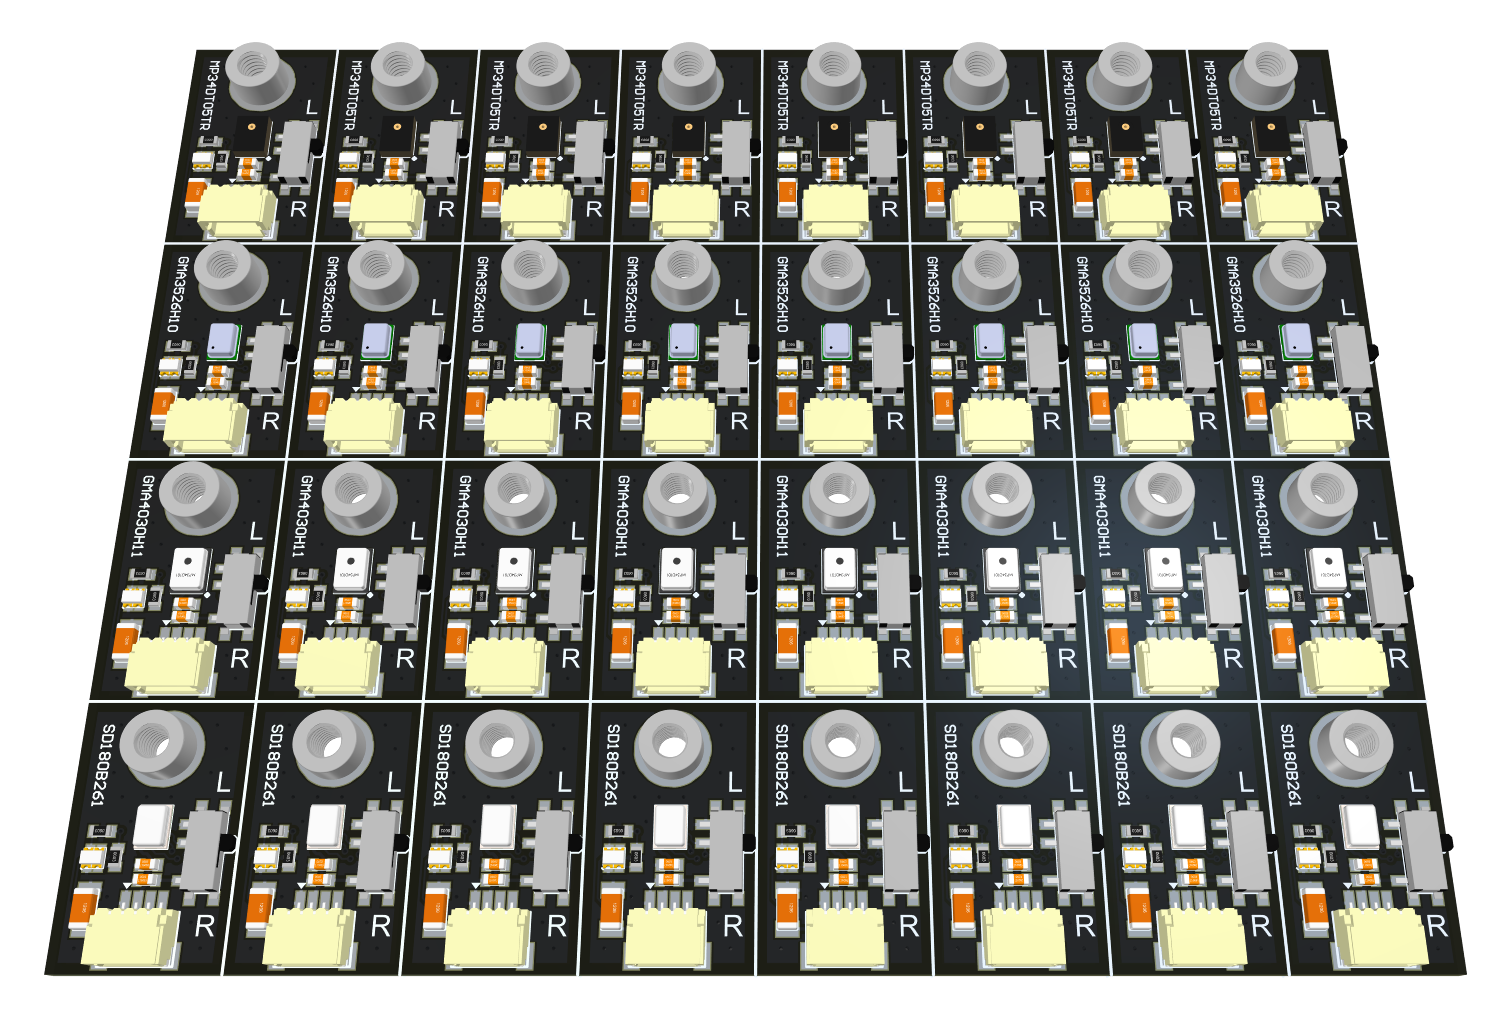
\includegraphics[width=0.85\textwidth]{images/4_design_acquisition_system/Microphone_Boards_Front.png}
	\caption{Front View of the Microphone Breakout-Boards}
	\label{fig:microphone_boards_front}
\end{figure}

Every microphone board is equipped with a slide switch for the channel selection, allowing to toggle between the left and right \acrshort{pdm} channel.
Additionally, a dual-color \acrshort{led} is integrated, serving as a power indicator. It lights up red if the right channel is selected or white if the left channel is selected.
To enhance the ease of mounting, each board includes a threaded surface-mounted standoff nut for an M3 screw, enabling straightforward attachment to a frame.

For connectivity, a standard SH\,4-Pin JST
\footnote{JST refers to Japan Solderless Terminal, a leading manufacturer of a diverse range of connectors, including wire-to-board, board-to-board, and wire-to-wire types.}
connector with a 1\,mm pin pitch was used.
This connector type is commonly found in \gls{adafruit} \textit{STEMMA QT / Qwiic JST} \acrshort{i2c} accessories boards.
By using this specific type, a wide range of pre-assembled cables with different lengths are available, simplifying the connection between the breakout boards and the acquisition system.
The microphone carrier \acrshort{pcb} follows the same pinout as \gls{adafruit}'s own \acrshort{pdm}-Microphone breakout board (\gls{adafruit} part number: 4346), facilitating compatibility.
The connector also supplies power (3.3V) to the microphones, allowing multiple units to be connected with a single cable.
For the testing setup, cables measuring 40 cm in length were used (\gls{adafruit} part number: 5385).
\begin{figure}[h!]
	\centering
	\begin{minipage}{0.49\textwidth}
		\centering
		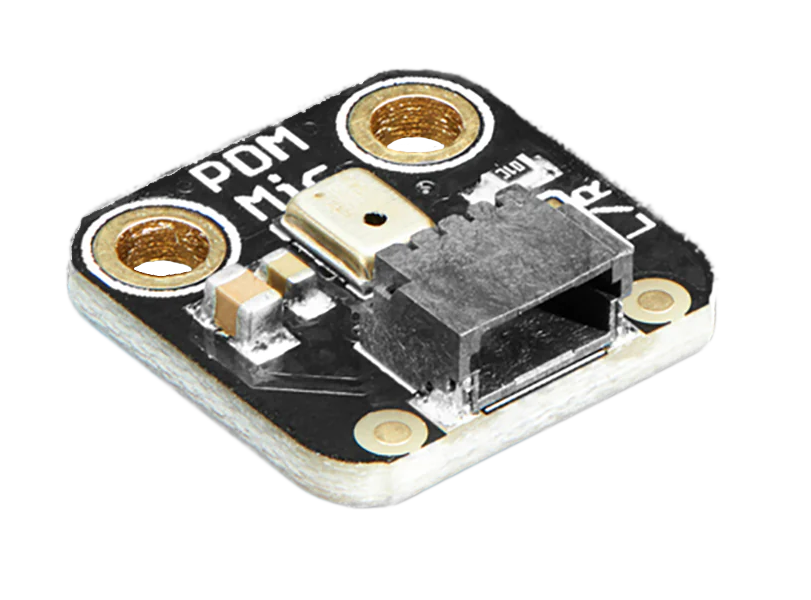
\includegraphics[height=4.0cm]{images/4_design_acquisition_system/adafruit_pdm_microphone.png}
		\caption{Adafruit PDM Microphone (4364)}
		\label{fig:adafruit_pdm_microphone}
	\end{minipage}
	\begin{minipage}{0.49\textwidth}
		\centering
		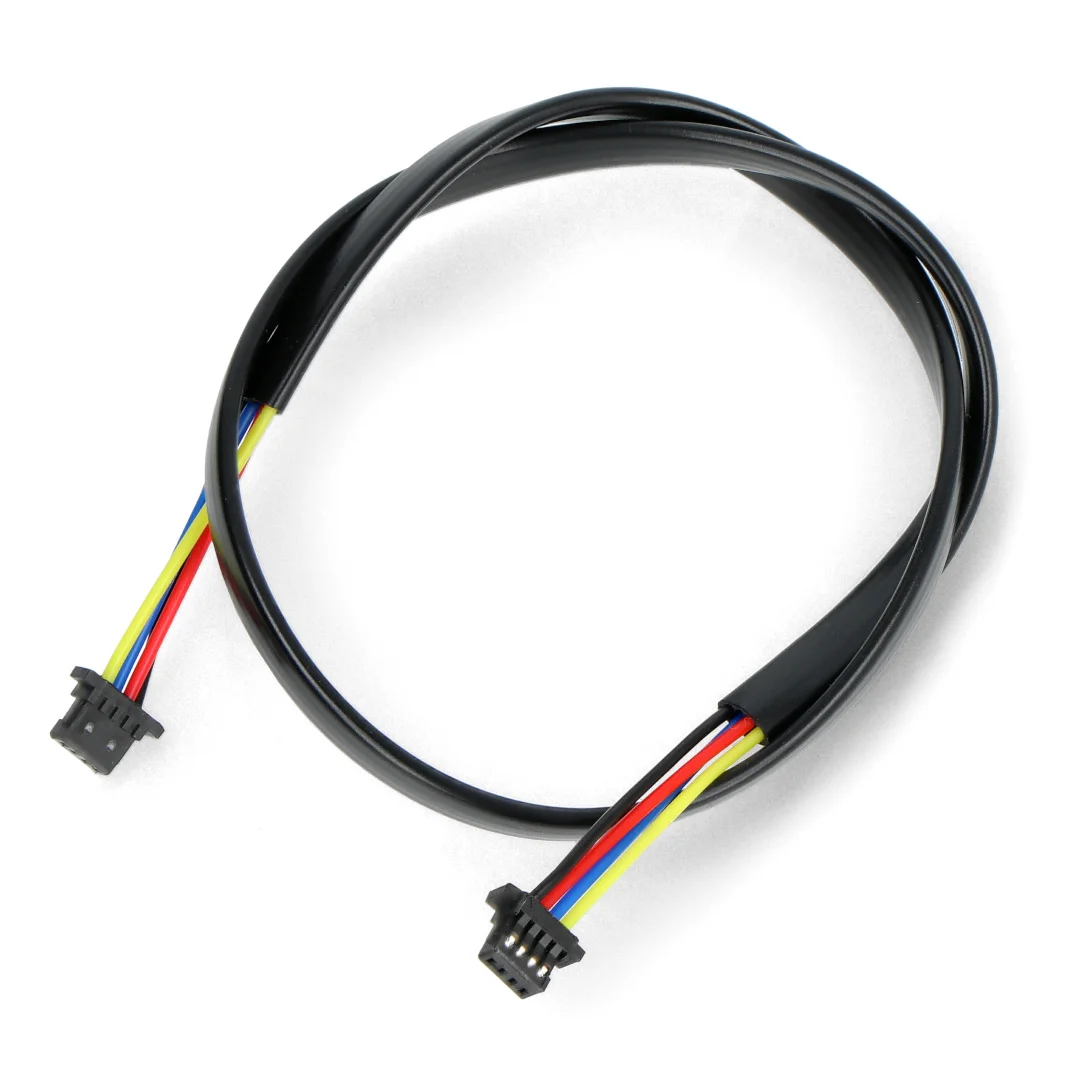
\includegraphics[height=4.0cm]{images/4_design_acquisition_system/stemma_qt_qwiic_cable.png}
		\caption{STEMMA QT / Qwiic Cable (5385)}
		\label{fig:stemma_qt_qwiic_cable}
	\end{minipage}
\end{figure}

The table below outlines the pinout used for these microphone breakout boards:
\begin{table}[h]
	\centering
	\begin{tabular}{|c|l|}
		\hline
		\textbf{Pin Number} & \textbf{Function}                    \\
		\hline
		1                   & GND                                  \\
		\hline
		2                   & 3V3                                  \\
		\hline
		3                   & PDM Data (provided by the host)      \\
		\hline
		4                   & PDM Clock (microphone output signal) \\
		\hline
	\end{tabular}
	\caption{Microphone Breakout Board Pinout}
	\label{tab:mic_breakout_pinout}
\end{table}

\newpage
\section{Hardware Design}
The hardware of the acquisition system is centralized around a 4-Layer \acrshort{pcb} with a size of 111.0\,mm x 136.0\,mm.
The connectors for the microphone breakout boards are located on the left and right side of the \acrshort{pcb} (16 channels on each side).
Each microphone channel is equipped with a pair of \acrshort{rgb} \acrshort{led}s.
The \acrshort{led} near the connector visually represents the audio level for its respective channel.
Another \acrshort{led}, situated on the white silk screen marking, indicates the active routing of the channel to the monitor headphones output.
A \textit{Monitor Selection} push button enables navigation through the microphone channels.
Each button press cycles through the channel numbers, directing the selected channel to the headphones output.
Additionally, a potentiometer is available for adjusting the volume of the headphones output.
On the lower segment of the \acrshort{pcb}, a 1.44" \acrshort{tft} touch display is embedded, serving as an interactive interface for controlling the acquisition system.
Adjacent to this display is the \textit{Record} button, which is used to start and stop the recording process.
The upper part of the device houses a \acrshort{usb} Type-C and an RJ45 connector, providing data connectivity to external devices.
Moreover, each corner of the \acrshort{pcb} is equipped with M3 surface-mounted standoff nuts, allowing for easy mounting of the acquisition system onto a microphone array frame.
\begin{figure}[h]
	\centering
	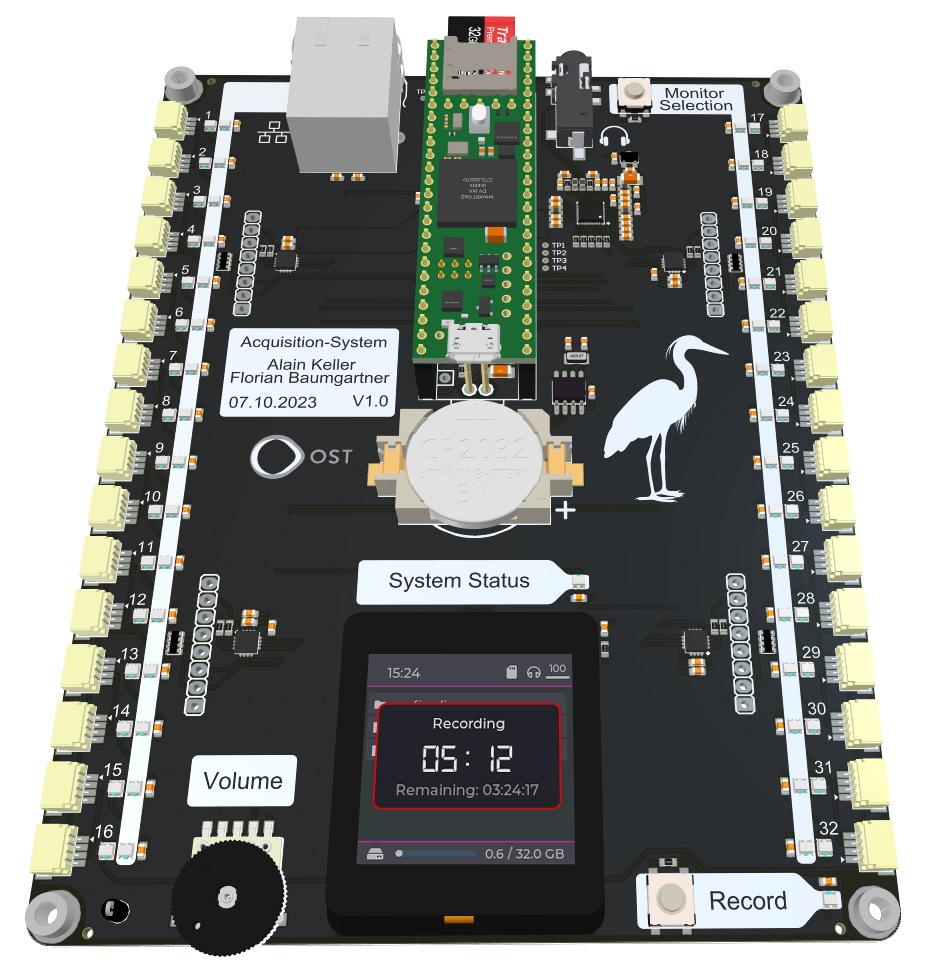
\includegraphics[width=0.92\textwidth, trim={0 0.5cm 0 0}]{images/4_design_acquisition_system/Acquisition_System_Front.png}
	\caption{Front View of the Acquisition System}
	\label{fig:acquisition_system_front}
\end{figure}
\newpage

\subsection{Block Diagram}
In figure \ref{fig:acquisition_system_design_block_diagram} the system block diagram is shown.
\vspace{-0.2cm}
\begin{figure}[h]
	\centering
	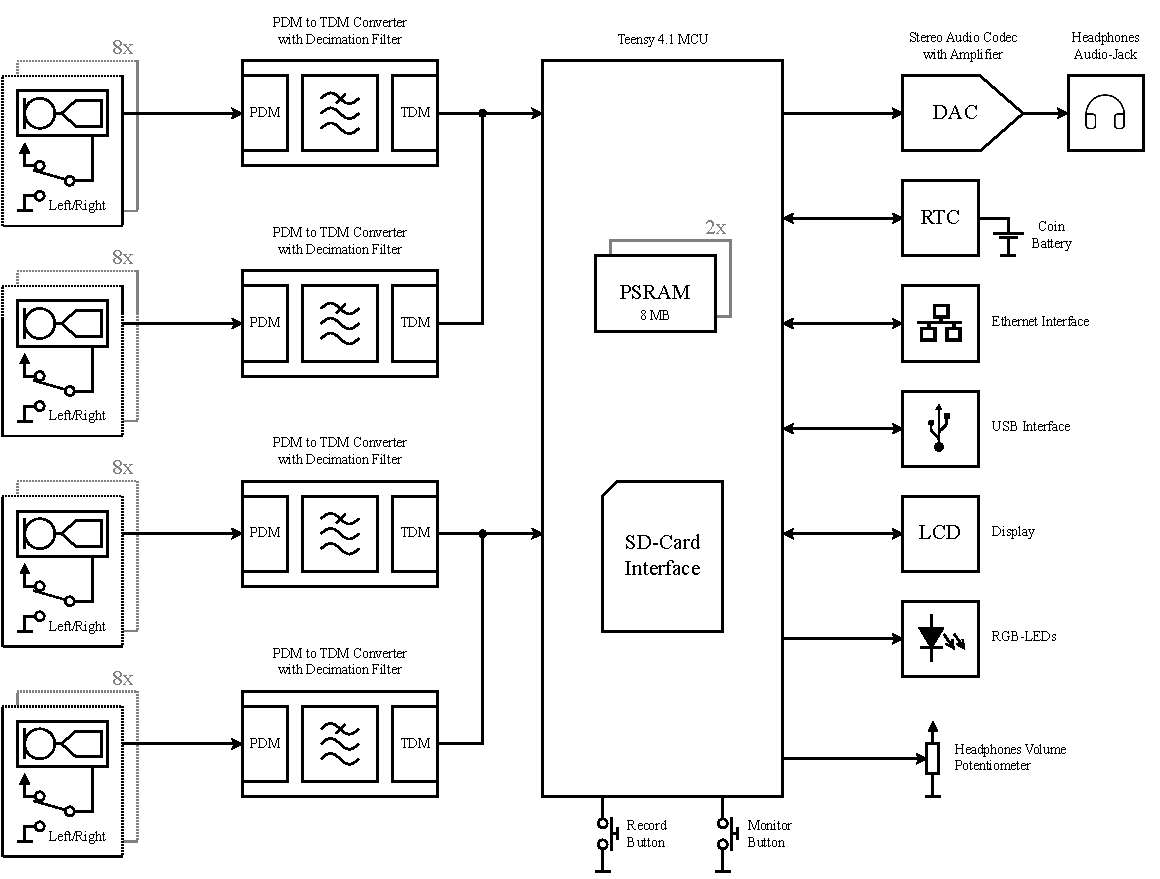
\includegraphics[width=1.0\textwidth, trim={0 0 0 0.1cm}]{images/4_design_acquisition_system/acquisition_system_design_block_diagram.pdf}
	\caption{System Block Diagram of Acquisition-System}
	\label{fig:acquisition_system_design_block_diagram}
\end{figure}
\vspace{-0.4cm}

\subsection{Microcontroller Unit (MCU)}
As a main \acrshort{mcu} the \texttt{Teensy 4.1} was chosen due to its powerful \acrshort{arm} Cortex-M7 processor, running at 600\,MHz.
The \texttt{Teensy 4.1} is a small form-factor development board, manufactured by \textit{PJRC}.
It provides a build-in programming interface, which allows to program the \acrshort{mcu} directly via \acrshort{usb} without the need for an external programmer.
Compared to the smaller formfactor \texttt{Teensy 4.0}, the \texttt{Teensy 4.1} includes a built-in \acrshort{sd}-Card holder and additional flash memory of 8\,MB.
Although the IMXRT1060 \acrshort{soc} provides 1\,MB of \acrshort{ram}, for this application, two additional 8\,MB \acrshort{psram} memory chips are required.
They can convenient be mounted on the backside of the \texttt{Teensy 4.1} board as shown in figure \ref{fig:teensy_psram}.
\begin{figure}[h!]
	\centering
	\begin{minipage}{0.49\textwidth}
		\centering
		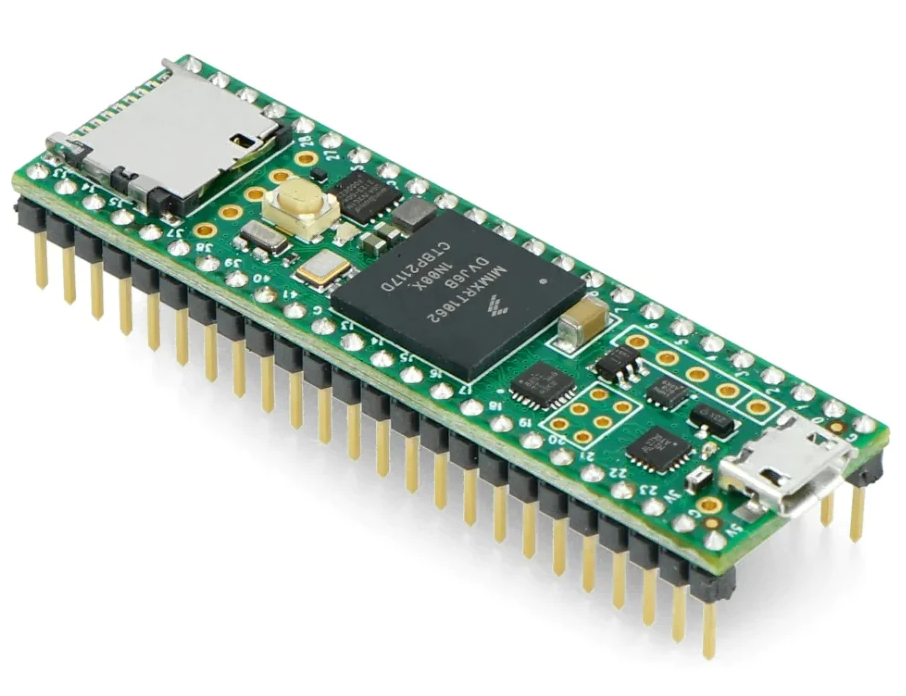
\includegraphics[height=3.7cm]{images/4_design_acquisition_system/teensy_image.png}
		\vspace{-0.2cm}
		\caption{Teensy 4.1}
		\label{fig:teensy_4_1}
	\end{minipage}
	\begin{minipage}{0.49\textwidth}
		\centering
		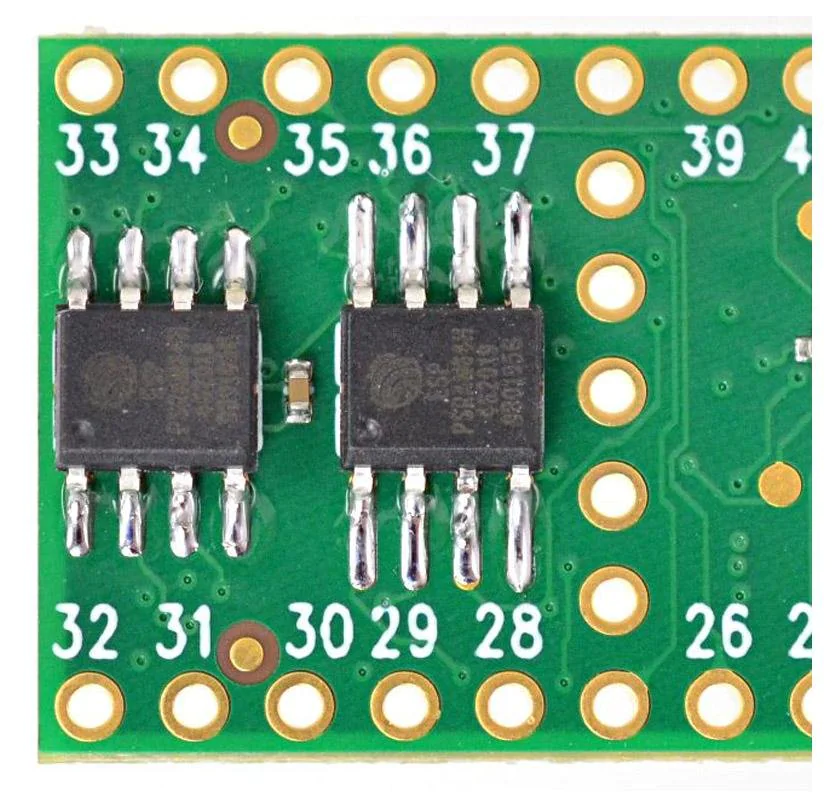
\includegraphics[height=3.7cm]{images/4_design_acquisition_system/teensy_psram.png}
		\vspace{-0.2cm}
		\caption{Mounting of external PSRAM}
		\label{fig:teensy_psram}
	\end{minipage}
\end{figure}
\newpage

\subsection{Audio Input}
As mentioned in section \ref{sec:pdm_microphones}, the use of \acrshort{pdm} microphones requires a digital decimation filter to convert their bitstream into a usable audio format.
The Teensy 4.1, despite having built-in hardware \acrshort{pdm} decimation, is limited to two channels, requiring external decimation for systems with more audio channels.

To overcome this limitation, the \textit{ADAU7118} from Analog Devices is employed.
This \acrfull{ic} is specialized in handling \acrshort{pdm} signals, offering four \acrshort{pdm} inputs and two clock outputs, which collectively can drive up to eight microphones in a multiplexed configuration.
It outputs audio data in the \acrshort{tdm} protocol.
\acrshort{tdm}-16, being capable of handling up to 16 channels, allows two \textit{ADAU7118} \acrshort{ic}s to share the same physical bus.
Hence, individual configuration is necessary to ensure that each converter accesses the correct \acrshort{tdm} slots (lower or upper 8 channels).
In total, four \textit{ADAU7118} \acrshort{ic}s are used, providing 32 microphone channels.

The \textit{ADAU7118} is also equipped with an \acrshort{i2c} interface, enabling the configuration of various parameters such as the decimation ratio,
\acrshort{tdm} bus settings, and signal drive impedances.


\subsection{Headphones Output}
The addition of a headphones output to the acquisition system introduces the capability for live monitoring of microphone inputs.
This feature allows a user to connect standard headphones with a 3.5\,mm jack directly to the device, enabling real-time audio feedback.

The system employs the \textit{WM8904} audio \acrshort{codec} as its \acrfull{dac}.
This choice is strategic, as the \textit{WM8904} not only supports digital audio input streams like \acrshort{i2s} and \acrshort{tdm},
but also includes a built-in headphones amplifier, making it particularly suitable for this application.
Additionally, its \acrshort{i2c} interface enables configuration adjustments, including device setup and volume control.

However, it is important to note that, as of this writing, this headphones output feature has not been implemented in the firmware.
Consequently, the hardware designed to support this functionality has not yet undergone testing.


\newpage
\section{Firmware Design}
The firmware is written in C++ and is based on the \gls{arduino} framework that has been addopted to the Teensy microcontroller environment.
As an \acrshort{ide}, the \acrshort{vscode} extension \textit{PlatfromIO} was used, as it provides powerful development tools and a great integration of the \gls{arduino} framework.

The firmware is divided into modules running in individual threads, facilitated by \textit{TeensyThreads} on the Teensy 4.1 microcontroller.
This lightweight multitasking library allows for concurrent execution of multiple threads, optimizing system performance and resource utilization.
\textit{TeensyThreads} has a minimal memory footprint and is optimized for efficient \acrshort{cpu} usage, making it ideal for embedded systems.
In total, 6 threads are running in parallel, as shown in table \ref{tab:acquisition_system_threads}.
\begin{table}[h]
	\centering
	\begin{tabular}{|l|l|}
		\hline
		Thread                     & Purpose                      \\ \hline
		\texttt{Console Interface} & Handles USB virtual COM-Port \\ \hline
		\texttt{Console Streaming} & Handles queuing of messages  \\ \hline
		\texttt{AudioUtils}        & Audio Processing             \\ \hline
		\texttt{HMI}               & LED Control \& RTC           \\ \hline
		\texttt{Application}       & Main Application Logic       \\ \hline
		\texttt{Main}              & Main Thread (Background)     \\ \hline
	\end{tabular}
	\caption{Overview of all Threads and their Purpose}
	\label{tab:acquisition_system_threads}
\end{table}

\subsection{Audio Recording}
The multichannel audio recording is achieved by a dual-context approach, focusing on capturing audio data and storing it on the \acrshort{sd}-Card.
While the capturing process is very time-critical and therefore runs at high priority, storing data on the \acrshort{sd}-Card can be done in the background.

\subsubsection{Audio Processing Pipeline}
The audio data is processed in blocks, where each block consists of 128 samples from each of the 32 microphone channels.
Upon capturing a new block, an \acrfull{irq} service routine is called by the Teensy Audio Library.
A critical step in processing is the interleaving of audio samples, as this is necessary to comply with the WAV file format.
This process rearranges the data from individual channels into a sequential stream, as visualized in Figure \ref{fig:audio_interleaving}.
\begin{figure}[h]
	\centering
	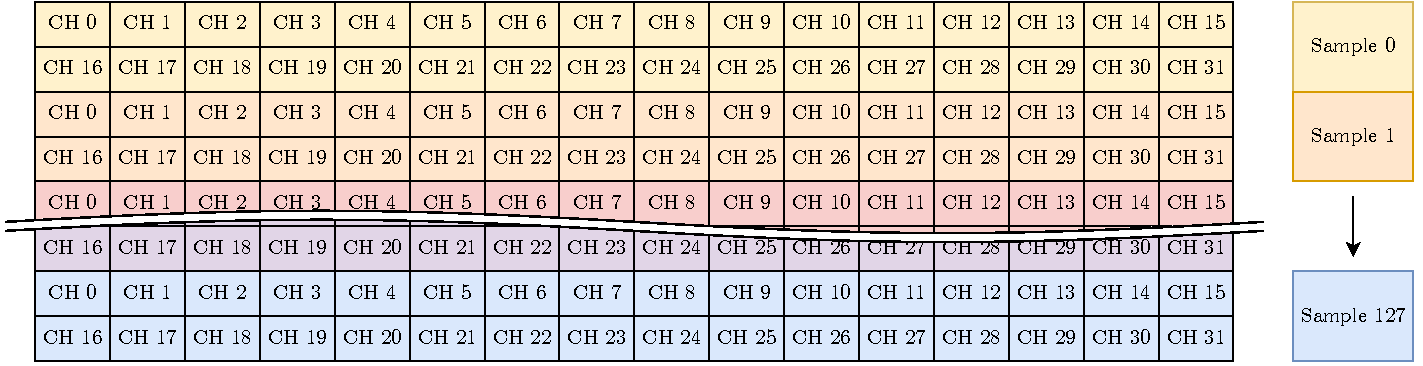
\includegraphics[width=1.0\textwidth]{images/4_design_acquisition_system/audio_interleaving.pdf}
	\caption{Interleaving of Audio Samples}
	\label{fig:audio_interleaving}
\end{figure}

\newpage
\subsubsection{SD-Card File Handling}
The interleaved audio data is then stored in a 12\,MB circular buffer located in the external \acrshort{psram}.
A background event handler regularly checks the buffer for new data, which, upon availability, is read and subsequently written to the current audio file on the \acrshort{sd}-Card.
Each writing operation also involves updating the WAV file header, a necessary step to maintain a valid file structure.

Given the complexities of \acrshort{sd}-Card operations, including variable access times and internal cache structures, the system is designed to verify each write operation.
In the event of incomplete data transfer, the process is reiterated until all data chunks are successfully written to the file.
Figure \ref{fig:acquisition_system_audio_recording_flow_diagram} shows a flow diagram of the audio recording process.
\begin{figure}[h]
	\centering
	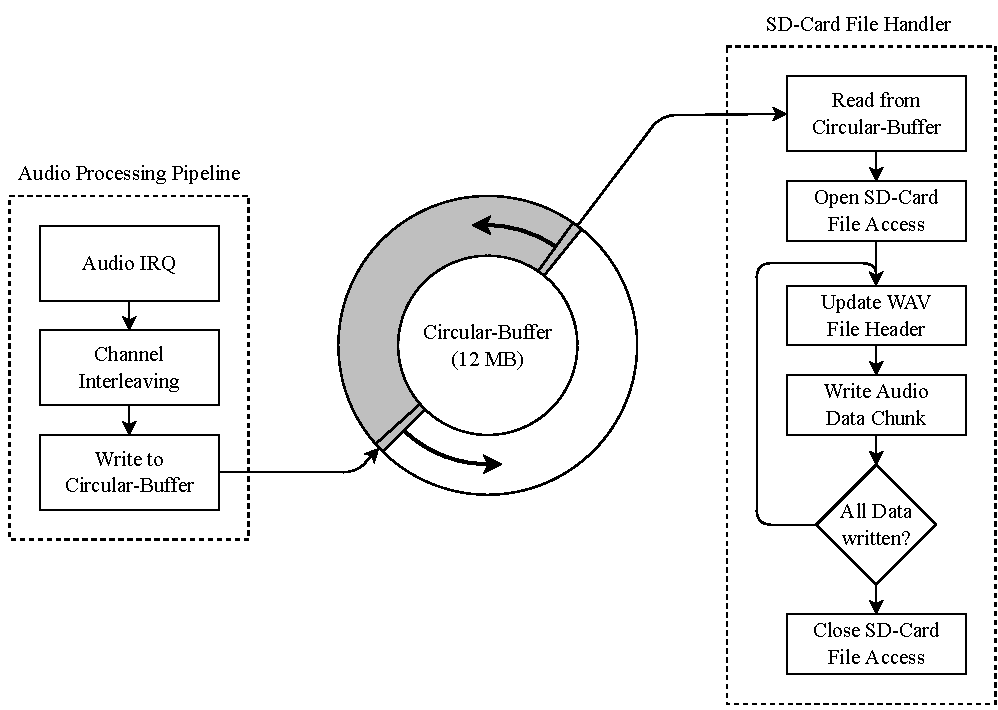
\includegraphics[width=1.0\textwidth, trim={0 0 0 0.5cm}]{images/4_design_acquisition_system/acquisition_system_audio_recording_flow_diagram.pdf}
	\caption{Flow Diagram of the Audio Recording Process}
	\label{fig:acquisition_system_audio_recording_flow_diagram}
\end{figure}

\subsubsection{File Naming Convention}
The convention for naming audio files is as follows:  \smallskip \newline
\texttt{YYMMDD\_HHMMSS\_<CH\_COUNT>\_<CH\_CONF>.wav} \smallskip \newline
This format incorporates the date and time of the recording, along with the channel count and configuration, thereby a straightforward file identification and organization is possible.
The chanel count is represented in decimal format, while the channel configuration is a 32-bit hexadecimal number, where each bit corresponds to a channel.
The \acrfull{lsb} represents channel 1, while the \acrfull{msb} represents channel 32.
If the bit is set to 1, the channel is active and therefore included in the recording.
The following file name example illustrates a 16 channel recording with channels 8 - 24 active:
\texttt{240118\_122417\_16\_00FFFF00.wav}


\newpage
\subsection{Graphical User Interface (GUI)}
The \acrshort{gui} provides a user-friendly interface for configuring the device and monitoring its status.
It is based on the \acrshort{lvgl} framework, which is described in detail in the next section.

\subsubsection{Light and Versatile Embedded Graphics Library (LVGL)}
\acrfull{lvgl} is a free and open-source graphics library, primarily used for creating embedded \acrshort{gui}s.
It's designed to be lightweight, consuming minimal memory and processing power, which is essential in embedded systems where resources are limited.

The decision to use \acrshort{lvgl} in conjunction with the \textit{NXP GuiGuider}, a graphical design tool, enables a rich set of features and enables rapid development.
\textit{GuiGuider} provides a user-friendly interface for designing \acrshort{gui}s, significantly simplifying the process of creating complex, visually appealing interfaces for embedded systems.
It provides a code generator, which generates the necessary C-Code to translate the graphic design into \acrshort{lvgl} \acrshort{api} calls.

\subsection{GUI Pages}
The \acrshort{gui} is minimalisticly designed and straight forward to use.
The navigation between the main pages is done by swiping left or right on the touchscreen.
Next, the individual pages are described in detail.

\begin{minipage}{\linewidth}
	\begin{wrapfigure}{l}{4.5cm}
		\vspace{-0.6cm}
		
\includegraphics[width=4cm]{images/4_design_acquisition_system/gui/01_splash_screen.png}
		\centering
		\caption{Splash Screen}
		\label{fig:acquisition_system_gui_splash_screen}
	\end{wrapfigure}
	\subsubsection{Splash Screen}
	When the device is powered on, the splash screen is displayed until the boot process is finished.
	On average this takes about 5 seconds.
\end{minipage}
\vspace{2.9cm}

\begin{minipage}{\linewidth}
	\begin{wrapfigure}{l}{4.5cm}
		\vspace{-0.6cm}
		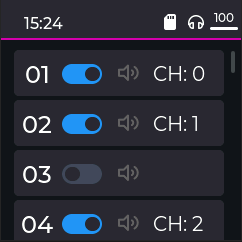
\includegraphics[width=4cm]{images/4_design_acquisition_system/gui/03_channel_settings.png}
		\centering
		\caption{Channel Settings}
		\label{fig:acquisition_system_gui_channel_settings}
	\end{wrapfigure}
	\subsubsection{Channel Settings}
	After the boot process is finished, the channel settings page is displayed.
	In the header bar located at the top of the page, the current time, \acrshort{usb} interface status, \acrshort{sd}-Card status and headphones volume are displayed.
	A list of all 32 microphone inputs is shown in the center of the page.
	Each input channel can be enabled or disabled by clicking on the corresponding switch.
	When an input is enabled, its associated channel number on the WAV file is displayed.
	A speaker symbol shows if the channel is currently routed to the headphones monitor output (green means active, grey means inactive).
\end{minipage}
\newpage

\begin{minipage}{\linewidth}
	\begin{wrapfigure}{l}{4.5cm}
		\vspace{-0.6cm}
		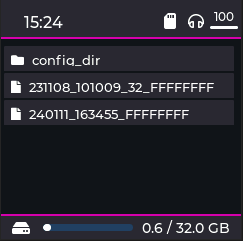
\includegraphics[width=4cm]{images/4_design_acquisition_system/gui/02_file_browser.png}
		\centering
		\caption{File Browser}
		\label{fig:acquisition_system_gui_file_browser}
	\end{wrapfigure}
	\subsubsection{File Browser}
	The file browser shows all files and folders located on the SD-Card.
	On the bottom of the page, a status bar indicates the current free and used space of the SD-Card.
	Due to the limited amount of memory, only the first 100 files and folders are displayed.
	This is however sufficient for most use cases.
\end{minipage}
\vspace{1.2cm}

\begin{minipage}{\linewidth}
	\begin{wrapfigure}{l}{4.5cm}
		\vspace{-0.6cm}
		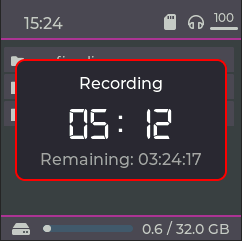
\includegraphics[width=4cm]{images/4_design_acquisition_system/gui/04_recording.png}
		\centering
		\caption{Recording}
		\label{fig:acquisition_system_gui_recording}
	\end{wrapfigure}
	\subsubsection{Recording}
	When the record button is pressed, the recording begins and a panel overlay is displayed.
	In the centre of the panel, the current recording time is displayed in minutes and seconds.
	Below, the remaining recording time is shown.
	When the recording is stopped, the panel overlay disappears.
	While the device is recording, all \acrshort{ui} elements and the navigation are disabled.
\end{minipage}
\vspace{0.7cm}

\begin{minipage}{\linewidth}
	\begin{wrapfigure}{l}{4.5cm}
		\vspace{-0.6cm}
		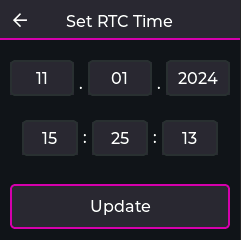
\includegraphics[width=4cm]{images/4_design_acquisition_system/gui/05_set_time.png}
		\centering
		\caption{Set RTC Time}
		\label{fig:acquisition_system_gui_set_time}
	\end{wrapfigure}
	\subsubsection{Set RTC Time}
	When the user clicks on the time in the header bar, the set time page is displayed.
	There the user can set the current time and date.
	After clicking on the \textit{Update} button, the new time is set and the page is closed.
	To abort the process, the user can click on the arrow in the header bar.
\end{minipage}
\clearpage
